\providecommand{\ecmpage}[1]{\clearpage\section*{\color{accent}#1}}
\topic{6a. ECM und Kalman-Filter Schritt für Schritt}
\label{ecm:start}
Dieses Lernkapitel verbindet das elektrische Ersatzschaltbild mit den Zustands-, Diskretisierungs- und Filtergleichungen der Dissertation. Es steht bewusst zwischen Kapitel 6 und 7 des Fragenkatalogs. Die bisherigen Kapitel- und Fragenummern bleiben erhalten.

\question{Was soll ich danach selbst nachrechnen können?}
\begin{enumerate}
\item Aus einem einfachen RC-Schaltbild zwei Differentialgleichungen und die Ausgangsspannung herleiten.
\item Aus der kontinuierlichen RC-Gleichung einen diskreten Rechenschritt ableiten und ihn von einer Euler-Näherung unterscheiden.
\item Zustand $x$, Eingang $u$, Ausgang $y$ und die Matrizen $A,B,C,D$ zeilenweise aufbauen; anschließend die Filtergrößen verstehen.
\item Einen vollständigen EKF-Schritt und seine Fortsetzung mit drei Zuständen von Hand nachvollziehen.
\item Erklären, welche Annahmen hinter der Spannungskorrektur stehen und was die konkrete Implementierung zusätzlich macht.
\end{enumerate}

\textbf{Modellumfang:} Der ECM-Einstieg (01--07) verwendet einen RC-Zweig mit zwei Zuständen. Der anschließende Kalman-Teil behandelt weiterhin das 2RC-Modell der Implementierung mit drei Zuständen. Dort steht $z$ für SOC und $C_b$ für $C_N$; die dortige diskrete Matrix $A$ entspricht dem hier eingeführten $A_d$.

\question{Die drei Ebenen der Erklärung}
\textbf{ECM:} Ein elektrisches Modell sagt voraus, wie sich SOC und Polarisationsspannungen unter einem Strom entwickeln und welche Klemmenspannung dazu gehört.

\textbf{Diskretisierung:} Der kontinuierliche Verlauf wird in eine Vorschrift für die Messzeitpunkte überführt. Das ist noch keine Korrektur mit einer Messung.

\textbf{Kalman-Filter:} Die vorhergesagte Klemmenspannung wird mit der gemessenen verglichen. Das Residuum korrigiert den inneren Zustand, gewichtet nach der angenommenen Unsicherheit.

\question{Lesereihenfolge}
\begin{tabular}{p{.12\linewidth}p{.79\linewidth}}
01--04 & Ein RC-Zweig, Differentialgleichungen, Zustandsraum und Aufbau von $A,B$.\\
05--07 & Ausgang $y$, Matrizen $C,D$, Diskretisierung und vollständiges Zahlenbeispiel.\\
08--12 & Filteridee, Kovarianzen, Matrizen und Herleitung des Kalman-Updates.\\
13--17 & Vollständig gerechnetes Drei-Zustands-Beispiel und zweiter Schritt.\\
18--24 & Tuning, Beobachtbarkeit, Codeabgleich, Übungen und Verteidigungsfragen.\\
\end{tabular}

\textbf{Kennzeichnung:} Die Zahlenbeispiele sind eigens gewählte Lehrwerte, keine nachträglich rekonstruierten Messergebnisse der Dissertation. Die tatsächlichen Codekonstanten stehen getrennt im Implementierungsabgleich. Dort wird auch eine Abweichung der implementierten Spannungsvorhersage von der üblichen Lehrbuchform ausdrücklich benannt.

\ecmpage{6a.01 -- Ein RC-Zweig: Schaltbild und Vorzeichen}
\label{ecm:circuit}
Wir verwenden die Bezeichnungen aus deiner Skizze: $\mathrm{SOC}$, $U_1$, $I$, $C_N$, $R_0$, $R_1$ und $C_1$. Ein RC-Zweig genügt, um den Weg zum Zustandsraum zu verstehen.
\begin{center}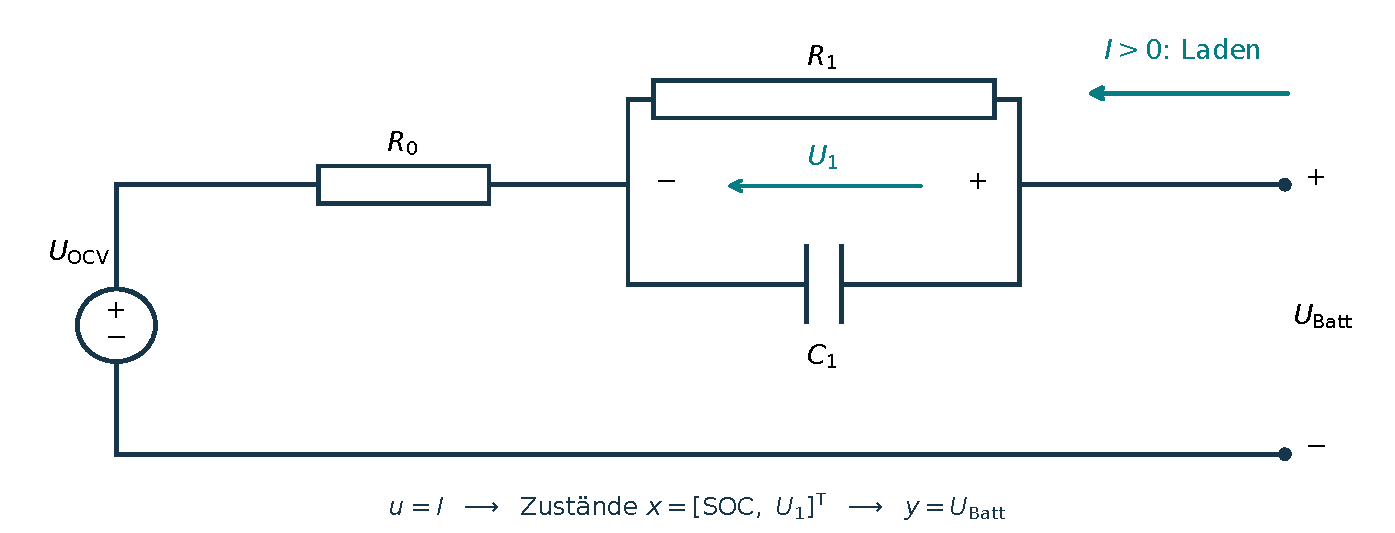
\includegraphics[width=\linewidth]{ecm_kalman/ecm_single_rc.pdf}\end{center}
\textbf{Konvention:} $I>0$ bedeutet Laden, $I<0$ Entladen. Die eingezeichneten Pluszeichen legen die Spannungsrichtungen fest. Damit gilt:
\[
\boxed{U_{\mathrm{Batt}}=U_{\mathrm{OCV}}(\mathrm{SOC})+R_0I+U_1.}
\]
$U_{\mathrm{Batt}}$ ist dieselbe Klemmenspannung, die du unten auf deinem Blatt als $U_K$ bezeichnest.

\begin{tabular}{p{.22\linewidth}p{.66\linewidth}}
\toprule Zeichen & Bedeutung\\\midrule
$U_{\mathrm{OCV}}$ & Ruhespannung als Funktion des SOC.\\[3pt]
$R_0$ & Ohmscher Serienwiderstand; sein Spannungsanteil ist $R_0I$.\\[3pt]
$R_1\parallel C_1$ & Paralleler Widerstand und Kondensator; beide haben die Spannung $U_1$.\\[3pt]
$C_N$ & Ladungskapazität der Batterie in Coulomb: $C_N=3600\,C_{N,\mathrm{Ah}}$.\\[3pt]
$C_1$ & Elektrische Kapazität des RC-Kondensators in Farad.\\\bottomrule
\end{tabular}

\question{Welche Größen sollen wir am Ende berechnen?}
\[
\underbrace{x=\begin{bmatrix}\mathrm{SOC}\\U_1\end{bmatrix}}_{\text{innere Zustände}}
\qquad
\underbrace{u=I}_{\text{Eingang}}
\qquad
\underbrace{y=U_{\mathrm{Batt}}}_{\text{Ausgang}}.
\]
Der Strom $u$ treibt das Modell an. Die Zustände $x$ tragen seine Vorgeschichte. Aus beiden entsteht die Ausgangsspannung $y$. Ein RC-Zweig bedeutet hier also \textbf{zwei Zustände}: SOC und Kondensatorspannung.

\textbf{Vereinfachung für diese Herleitung:} konstante Parameter und Coulomb-Wirkungsgrad $\eta=1$. Der SOC wird als Bruchteil gerechnet: $0{,}60$ entspricht 60 Prozent. Das Schaltbild ist ein Ersatzmodell, kein wörtlicher Aufbau der Zellchemie.

\ecmpage{6a.02 -- Die zwei Differentialgleichungen herleiten}
\question{1. SOC: Strom verändert die gespeicherte Ladung}
Mit Ladung $q$ und konstanter Batteriekapazität $C_N$:
\[
\mathrm{SOC}=\frac{q}{C_N},\qquad \dot q=I
\quad\Longrightarrow\quad
\boxed{\dot{\mathrm{SOC}}=\frac{1}{C_N}I.}
\]
Als Integral, genau wie auf deinem Blatt:
\[
\mathrm{SOC}(t)=\mathrm{SOC}(t_0)+\frac{1}{C_N}\int_{t_0}^{t}I(s)\,\mathrm ds.
\]
Ein Punkt über einer Größe bedeutet ihre Ableitung nach der Zeit. Für Zeit in Sekunden muss $C_N$ in Coulomb eingesetzt werden; beispielsweise 2 Ah $=7200$ C.

\question{2. RC-Zweig: den Strom auf Widerstand und Kondensator aufteilen}
Wegen der Parallelschaltung liegt an beiden Bauteilen dieselbe Spannung $U_1$:
\[
\underbrace{I=I_{R_1}+I_{C_1}}_{\text{Knotenregel}},\qquad
\underbrace{I_{R_1}=\frac{U_1}{R_1}}_{\text{Ohmsches Gesetz}},\qquad
\underbrace{I_{C_1}=C_1\dot U_1}_{\text{Kondensatorgleichung}}.
\]
\textbf{Einsetzen, dann nach $\dot U_1$ umstellen:}
\[
\begin{aligned}
I&=\frac{U_1}{R_1}+C_1\dot U_1,\\[4pt]
C_1\dot U_1&=I-\frac{U_1}{R_1},\\[4pt]
\dot U_1&=\frac{1}{C_1}I-\frac{1}{R_1C_1}U_1.
\end{aligned}
\]
\[
\boxed{\dot U_1=-\frac{1}{R_1C_1}U_1+\frac{1}{C_1}I.}
\]
Der erste Term beschreibt das Abklingen der bisherigen Spannung, der zweite den Einfluss des Stroms. Ohne Strom fällt $U_1$ gegen null; bei konstantem Strom nähert es sich $R_1I$.

\question{3. Die Ausgangsspannung folgt aus der Maschenregel}
\[
\boxed{y=U_{\mathrm{Batt}}=U_{\mathrm{OCV}}(\mathrm{SOC})+R_0I+U_1.}
\]
Damit haben wir \textbf{zwei Gleichungen für die Zustandsänderungen} und \textbf{eine für den Ausgang}. Beim Entladen ist $I$ negativ; nach hinreichend langer Entladung ist auch $U_1$ negativ. Die Klemmenspannung liegt dann unter der Ruhespannung.

\ecmpage{6a.03 -- Was bedeuten x, u, y und A, B, C, D?}
\question{Zustandsraum heißt: dieselben Gleichungen geordnet aufschreiben}
Für ein lineares System lautet die übliche Form:
\[
\boxed{\dot x=Ax+Bu},\qquad \boxed{y=Cx+Du}.
\]
Die erste Gleichung beschreibt die \textbf{Entwicklung des Zustands}, die zweite den \textbf{Ausgang}. Beim ECM ist die OCV allgemein nichtlinear. Deshalb lautet seine Ausgangsgleichung zunächst $y=h(x,u)$. Die korrekte lokale Form mit $C,D$ und Spannungsoffset folgt auf 6a.05.

\question{Unsere Vektoren und Größen}
\[
x=\begin{bmatrix}\mathrm{SOC}\\U_1\end{bmatrix},\quad
\dot x=\begin{bmatrix}\dot{\mathrm{SOC}}\\\dot U_1\end{bmatrix},\quad
u=I,\quad y=U_{\mathrm{Batt}}.
\]
Die Reihenfolge ist fest: \textbf{erste Zeile SOC, zweite Zeile $U_1$}. $x$ ist ein Spaltenvektor mit zwei Einträgen. $u$ und $y$ sind hier jeweils eine einzelne Zahl.

\begin{tabular}{p{.10\linewidth}p{.18\linewidth}p{.60\linewidth}}
\toprule Matrix & Größe & Was macht sie?\\\midrule
$A$ & $2\times2$ & Systemmatrix: Wie beeinflussen die aktuellen Zustände ihre zeitlichen Änderungen?\\[7pt]
$B$ & $2\times1$ & Eingangsmatrix: Wie wirkt der Strom auf jede der beiden Zustandsänderungen?\\[7pt]
$C$ & $1\times2$ & Ausgangsmatrix: Wie wirken die Zustände auf die Ausgangsspannung, nach der gewählten Linearisierung?\\[7pt]
$D$ & $1\times1$ & Durchgriffsmatrix (in der Übung: Durchgangsmatrix): Welcher Spannungsanteil entsteht unmittelbar durch den Eingangsstrom?\\\bottomrule
\end{tabular}

\question{Warum genau diese Matrixgrößen?}
\[
\underbrace{A}_{2\times2}\underbrace{x}_{2\times1}
+\underbrace{B}_{2\times1}\underbrace{u}_{1\times1}
=\underbrace{\dot x}_{2\times1},
\]
\[
\underbrace{C}_{1\times2}\underbrace{x}_{2\times1}
+\underbrace{D}_{1\times1}\underbrace{u}_{1\times1}
=\underbrace{y}_{1\times1}\quad\text{(lineare Form)}.
\]
\textbf{Merksatz:} Jede Zeile von $A$ und $B$ gehört zu einer Zustandsgleichung. Die eine Zeile von $C$ und $D$ gehört zur einen Ausgangsgleichung.

\textbf{Achtung bei den Buchstaben:} $C$ ist eine Matrix, $C_1$ ein Kondensatorwert und $C_N$ die Batteriekapazität. $u$ ist der Eingangsstrom; das große $U_1$ ist eine Spannung.

{\small\textbf{Abgleich mit deinen Unterlagen:} SDB, Übung 4 -- Model-Based State Estimation, Aufgabe 2c--g, verwendet dieselben Bezeichnungen und Vorzeichen. MSB, Übung 2, Aufgabe 1a--c, verwendet dafür $R_1$ bzw. $R_2,C_2,U_2$. Die SDB-Übung 5 setzt auf diesem Zustandsmodell auf.}


\ecmpage{6a.04 -- A und B entstehen Zeile für Zeile}
\question{1. Zeile: die SOC-Gleichung nach SOC, U1 und I sortieren}
\[
\dot{\mathrm{SOC}}=\frac{1}{C_N}I
=\underbrace{0}_{a_{11}}\,\mathrm{SOC}
+\underbrace{0}_{a_{12}}\,U_1
+\underbrace{\frac{1}{C_N}}_{b_1}\,I.
\]
Also: erste Zeile von $A$: $\begin{bmatrix}0&0\end{bmatrix}$; erster Eintrag von $B$: $1/C_N$.
Die Nullen bedeuten: Bei festem $C_N$ hängt die \emph{SOC-Änderung} direkt vom Strom ab, nicht vom aktuellen SOC oder von $U_1$. Sie bedeuten nicht, dass SOC oder $U_1$ null wären.

\question{2. Zeile: die RC-Gleichung in derselben Reihenfolge sortieren}
\[
\dot U_1=-\frac{1}{R_1C_1}U_1+\frac{1}{C_1}I
=\underbrace{0}_{a_{21}}\,\mathrm{SOC}
+\underbrace{\left(-\frac{1}{R_1C_1}\right)}_{a_{22}}\,U_1
+\underbrace{\frac{1}{C_1}}_{b_2}\,I.
\]
Also: zweite Zeile von $A$: $\begin{bmatrix}0&-1/(R_1C_1)\end{bmatrix}$; zweiter Eintrag von $B$: $1/C_1$.

\question{3. Die beiden Zeilen untereinander setzen}
\[
\begin{array}{c|cc|c}
 &\text{Faktor vor SOC}&\text{Faktor vor }U_1&\text{Faktor vor }I\\\hline
\dot{\mathrm{SOC}}&0&0&1/C_N\\[5pt]
\dot U_1&0&-1/(R_1C_1)&1/C_1
\end{array}
\]
\[
\boxed{A=\begin{bmatrix}0&0\\[3pt]0&-1/(R_1C_1)\end{bmatrix}},
\qquad
\boxed{B=\begin{bmatrix}1/C_N\\[3pt]1/C_1\end{bmatrix}}.
\]

\question{4. Zur Kontrolle wieder ausmultiplizieren}
\[
\underbrace{\begin{bmatrix}\dot{\mathrm{SOC}}\\\dot U_1\end{bmatrix}}_{\dot x}
=
\underbrace{\begin{bmatrix}0&0\\0&-1/(R_1C_1)\end{bmatrix}}_A
\underbrace{\begin{bmatrix}\mathrm{SOC}\\U_1\end{bmatrix}}_x
+
\underbrace{\begin{bmatrix}1/C_N\\1/C_1\end{bmatrix}}_B
\underbrace{I}_u.
\]
Zeile mal Spalte liefert wieder beide Differentialgleichungen. Die Ausgangsspannung $y$ kommt als eigene Gleichung hinzu.

\question{5. Derselbe Ablauf als Signalfluss}
\begin{center}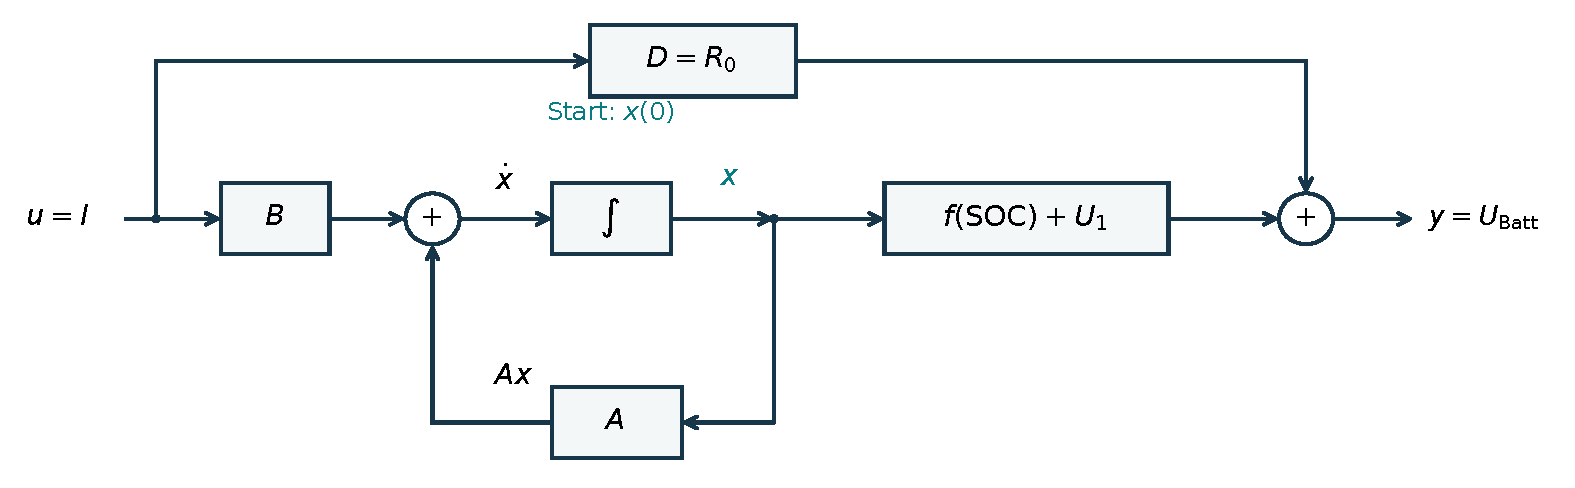
\includegraphics[width=\linewidth]{ecm_kalman/ecm_signal_flow.pdf}\end{center}
Integration mit dem Startwert $x(0)$ macht aus $\dot x$ den Zustand $x$.


\ecmpage{6a.05 -- Die Ausgangsgleichung: y, C und D}
\question{1. Erst die vollständige physikalische Gleichung}
\[
\boxed{y=U_{\mathrm{OCV}}(\mathrm{SOC})+1\cdot U_1+R_0\cdot u.}
\]
Wir kürzen $f(\mathrm{SOC})=U_{\mathrm{OCV}}(\mathrm{SOC})$ ab. Die RC-Spannung geht mit dem Faktor 1 ein; der direkte Stromanteil hat den Faktor $R_0$.

\question{2. Genau die Schreibweise aus deiner Skizze und der MSB-Übung}
Für $\mathrm{SOC}\ne0$ kann man den OCV-Term als Produkt schreiben:
\[
f(\mathrm{SOC})=\frac{f(\mathrm{SOC})}{\mathrm{SOC}}\cdot\mathrm{SOC}.
\]
Damit entsteht die \textbf{eine Ausgangszeile}:
\[
\underbrace{y}_{\text{Ausgang}}
=\underbrace{\begin{bmatrix}\dfrac{f(\mathrm{SOC})}{\mathrm{SOC}}&1\end{bmatrix}}_{C(x)}
\underbrace{\begin{bmatrix}\mathrm{SOC}\\U_1\end{bmatrix}}_x
+\underbrace{\begin{bmatrix}R_0\end{bmatrix}}_D\underbrace{I}_u.
\]
Ausmultiplizieren ergibt $[f(\mathrm{SOC})/\mathrm{SOC}]\,\mathrm{SOC}+U_1+R_0I$, also genau die Spannung aus Schritt 1.

\textbf{Was muss man dabei dazusagen?} Diese Matrix $C(x)$ hängt vom SOC ab. Die Schreibweise macht das Modell \emph{nicht linear}. Bei SOC null ist der Quotient nicht definiert; die ursprüngliche Funktion $f(0)$ kann trotzdem eine endliche Ruhespannung liefern. Deshalb ist $y=f(\mathrm{SOC})+U_1+R_0u$ die saubere allgemeine Ausgangsgleichung.

\question{3. Wenn C eine konstante lokale Ausgangsmatrix sein soll}
Um einen Bezugspunkt $s_\ast$ wird die OCV-Kurve durch ihre Tangente ersetzt:
\[
c=f'(s_\ast),\qquad
f(\mathrm{SOC})\approx f(s_\ast)+c(\mathrm{SOC}-s_\ast)
=c\,\mathrm{SOC}+\underbrace{f(s_\ast)-c\,s_\ast}_{e}.
\]
Wieder die Faktoren vor SOC, $U_1$ und $u$ ablesen:
\[
y\approx c\,\mathrm{SOC}+1\cdot U_1+R_0u+e,
\]
\[
\boxed{C_{\mathrm{lin}}=\begin{bmatrix}c&1\end{bmatrix}},\quad
\boxed{D=\begin{bmatrix}R_0\end{bmatrix}},\quad
\boxed{y\approx C_{\mathrm{lin}}x+Du+e}.
\]
Hier ist $c$ die \textbf{Steigung}, nicht der Quotient aus Schritt 2. Der Spannungsoffset $e$ gehört bei absoluten Größen dazu. Nur für Abweichungen vom Bezugspunkt entfällt er: $\delta y\approx C_{\mathrm{lin}}\delta x+D\delta u$.

\textbf{Das vollständige allgemeine Modell lautet damit:}
\[
\boxed{\dot x=Ax+Bu,\qquad y=f(\mathrm{SOC})+U_1+R_0u.}
\]
Schritt 2 ist eine exakte, zustandsabhängige Umschreibung für SOC ungleich null. Schritt 3 ist eine lokale lineare Näherung; bei einer tatsächlich geraden OCV ist sie exakt.

\textbf{Brücke zum Filter:} Die Mess-Jacobi-Matrix des EKF enthält die OCV-\emph{Steigung} $f'(\mathrm{SOC})$, nicht den Quotienten $f(\mathrm{SOC})/\mathrm{SOC}$. Auch wenn die Übung den Quotienten als zeitvariable Matrix schreibt, ist er keine Taylor-Linearisierung.

\ecmpage{6a.06 -- Von kontinuierlich zu diskret: A und B werden Ad und Bd}
\question{1. Messzeitpunkte statt einer zeitlichen Ableitung}
$x_k=x(t_k)$ und $\Delta t=t_{k+1}-t_k$. Zwischen zwei Zeitpunkten halten wir $u_k=I_k$ und die Bauteilparameter konstant. Gesucht ist $x_{k+1}$ aus $x_k$.

\question{2. SOC über den Schritt integrieren}
\[
\mathrm{SOC}_{k+1}-\mathrm{SOC}_k=\int_{t_k}^{t_{k+1}}\frac{u_k}{C_N}\,\mathrm dt
=\frac{\Delta t}{C_N}u_k.
\]

\question{3. Die RC-Gleichung lösen}
Mit $\tau=R_1C_1$ und der Zeit $s$ seit Schrittbeginn lautet sie
\[
\dot U_1+\frac{U_1}{\tau}=\frac{u_k}{C_1}.
\]
Mit $e^{s/\tau}$ multiplizieren und integrieren:
\[
\frac{\mathrm d}{\mathrm ds}(e^{s/\tau}U_1)=\frac{u_k}{C_1}e^{s/\tau}
\quad\Longrightarrow\quad
 e^{\Delta t/\tau}U_{1,k+1}-U_{1,k}=R_1u_k(e^{\Delta t/\tau}-1).
\]
Durch $e^{\Delta t/\tau}$ teilen. Mit $a=e^{-\Delta t/(R_1C_1)}$ folgt:
\[
\boxed{U_{1,k+1}=aU_{1,k}+R_1(1-a)u_k.}
\]

\question{4. Wieder die Faktoren zeilenweise in Matrizen schreiben}
\[
\boxed{x_{k+1}=A_dx_k+B_du_k},\quad
\boxed{A_d=\begin{bmatrix}1&0\\0&a\end{bmatrix}},\quad
\boxed{B_d=\begin{bmatrix}\Delta t/C_N\\R_1(1-a)\end{bmatrix}}.
\]
In der ersten Zeile steht jetzt eine Eins: Der bisherige SOC wird zum nächsten Zeitpunkt übernommen. Die Null in $A$ bezog sich dagegen auf seine \emph{Ableitung}.
Die allgemeine Schreibweise aus der SDB-Übung liefert dasselbe Ergebnis:
\[
A_d=e^{A\Delta t},\qquad B_d=\int_0^{\Delta t}e^{As}B\,\mathrm ds.
\]
$e^{As}$ ist das Matrixexponential; hier gilt $e^{As}=\operatorname{diag}(1,e^{-s/(R_1C_1)})$.

\question{5. Der Ausgang bleibt Teil des diskreten Modells}
\[
\boxed{y_k=U_{\mathrm{OCV}}(\mathrm{SOC}_k)+U_{1,k}+R_0u_k}
\qquad (\text{lokal: } y_k\approx C_{\mathrm{lin}}x_k+Du_k+e).
\]
$y_k$ wird aus Zustand und Strom \emph{am Zeitpunkt $t_k$} berechnet; $x_{k+1}$ ist der daraus fortgeschriebene Zustand. Die Ausgangsgleichung wird nicht integriert.

\textbf{Euler wäre eine andere Diskretisierung:}
$A_{d,\mathrm E}=\mathsf I+\Delta t A$, $B_{d,\mathrm E}=\Delta t B$. Dabei ersetzt $1-\Delta t/(R_1C_1)$ den Exponentialfaktor $a$. Die obige Lösung ist unter der Konstanthaltungsannahme exakt; Euler ist eine Näherung. $\mathsf I$ bezeichnet hier die Einheitsmatrix.

\ecmpage{6a.07 -- Ein kompletter Rechenschritt bis zur Ausgangsspannung}
\question{1. Einfache Lehrwerte festlegen}
\[
C_N=2\,\mathrm{Ah}=7200\,\mathrm C,\quad R_0=0{,}03\,\Omega,\quad
R_1=0{,}04\,\Omega,\quad C_1=500\,\mathrm F.
\]
Damit ist $\tau=R_1C_1=20$ s. Wir starten mit $\mathrm{SOC}_0=0{,}60$, $U_{1,0}=0$ V und laden 5 s lang mit $u=I=1$ A. Für das Beispiel wählen wir die Gerade
\[
U_{\mathrm{OCV}}(\mathrm{SOC})=3{,}0+0{,}5\,\mathrm{SOC}\quad\text{in Volt}.
\]

\question{2. Alle vier kontinuierlichen Matrizen angeben}
\[
A=\begin{bmatrix}0&0\\0&-0{,}05\end{bmatrix},\quad
B=\begin{bmatrix}1/7200\\0{,}002\end{bmatrix},\quad
C_{\mathrm{lin}}=\begin{bmatrix}0{,}5&1\end{bmatrix},\quad D=\begin{bmatrix}0{,}03\end{bmatrix}.
\]
\[
\dot x=Ax+Bu,\qquad \boxed{y=C_{\mathrm{lin}}x+Du+3{,}0}.
\]
Am Anfang ist $y_0=0{,}5\cdot0{,}60+0+0{,}03\cdot1+3{,}0=3{,}33$ V.

\question{3. Die diskreten Matrizen für 5 Sekunden bilden}
\[
a=e^{-5/20}=0{,}778800783,
\]
\[
A_d=\begin{bmatrix}1&0\\0&0{,}778800783\end{bmatrix},\qquad
B_d=\begin{bmatrix}5/7200\\0{,}04(1-0{,}778800783)\end{bmatrix}
\approx\begin{bmatrix}0{,}000694444\\0{,}008847969\end{bmatrix}.
\]

\question{4. Die neuen Zustände berechnen: Zeile mal Spalte}
\[
x_1=A_dx_0+B_du_0
=\begin{bmatrix}1\cdot0{,}60+0\cdot0\\0\cdot0{,}60+0{,}778800783\cdot0\end{bmatrix}
+\begin{bmatrix}0{,}000694444\\0{,}008847969\end{bmatrix}\cdot1
\approx\boxed{\begin{bmatrix}0{,}600694444\\0{,}008847969\end{bmatrix}}.
\]
Der SOC beträgt 60,069444 Prozent, die RC-Spannung 8,847969 mV.

\question{5. Jetzt wirklich bis y weiterrechnen}
Der Strom sei auch am neuen Zeitpunkt weiterhin $u_1=1$ A:
\[
\begin{aligned}
y_1&=C_{\mathrm{lin}}x_1+Du_1+3{,}0\\
&=0{,}5\cdot0{,}600694444+1\cdot0{,}008847969+0{,}03\cdot1+3{,}0\\
&\approx\boxed{3{,}339195\,\mathrm V}.
\end{aligned}
\]
\textbf{Kontrolle über das Schaltbild:} $U_{\mathrm{OCV}}=3{,}300347$ V, $U_1=0{,}008848$ V und $R_0I=0{,}030000$ V. Ihre Summe ergibt denselben Ausgang $y_1$. Damit sind Zustand \emph{und} Ausgang berechnet.

\ecmpage{6a.08 -- Die Filteridee zuerst mit nur einer Zahl}
\question{Warum überhaupt korrigieren?}
Die Stromintegration liefert eine Vorhersage, aber Start-SOC, Strommessung, Kapazität und Modellparameter sind nicht perfekt bekannt. Die Spannungsmessung liefert zusätzliche Information. Der Filter verbindet beide Informationsquellen entsprechend ihrer Unsicherheit. Er kennt dabei weder den wahren SOC noch den tatsächlichen aktuellen Schätzfehler.

\question{Ein absichtlich vereinfachtes Beispiel}
Nur auf dieser Seite nehmen wir einen fiktiven Sensor an, der den SOC direkt misst. Die Modellvorhersage sei $\hat z^-=0{,}60$, die Messung $y=0{,}70$. Wir setzen an:
\[
\hat z^+=\hat z^-+K(y-\hat z^-)=(1-K)\hat z^-+Ky.
\]
$K=0$ vertraut nur der Vorhersage, $K=1$ nur der Messung. Gesucht ist ein sinnvoller Wert dazwischen. Im echten ECM ist die Messgröße dagegen eine Spannung; dort wird der Zusammenhang über die Messfunktion hergestellt.

\question{Woher kommt der optimale Faktor?}
Vorhersagefehler und Messrauschen seien unkorreliert und mittelwertfrei. Ihre Varianzen seien $P^-$ und $R$. Dann hat der korrigierte Fehler die Varianz
\[
P^+(K)=(1-K)^2P^-+K^2R.
\]
Wir minimieren sie durch Ableiten:
\[
\frac{\mathrm dP^+}{\mathrm dK}=-2(1-K)P^-+2KR=0
\quad\Longrightarrow\quad
\boxed{K=\frac{P^-}{P^-+R}}.
\]
Die zweite Ableitung ist $2(P^-+R)>0$: Es ist ein Minimum. Das Verhältnis entsteht aus einer Rechnung mit Unsicherheiten, nicht aus einer frei gewählten Mischung von 50 zu 50.

\question{Einmal vollständig einsetzen}
Modell-Standardabweichung: 5 Prozentpunkte, also $P^-=(0{,}05)^2=0{,}0025$. Sensor-Standardabweichung: 2,5 Prozentpunkte, also $R=(0{,}025)^2=0{,}000625$.
\[
K=\frac{0{,}0025}{0{,}0025+0{,}000625}=0{,}8,
\qquad \hat z^+=0{,}60+0{,}8\cdot0{,}10=0{,}68.
\]
\[
P^+=(1-K)P^-=0{,}0005,
\qquad \sigma^+=\sqrt{P^+}=0{,}02236.
\]
Das Ergebnis lautet 68 Prozent SOC mit einer modellierten Standardabweichung von etwa 2,24 Prozentpunkten. Das ist keine Garantie, dass der reale Fehler genau so groß ist.

\textbf{Übertragung:} Im ECM werden gleichzeitig drei Zustände korrigiert, obwohl nur eine Spannung gemessen wird. Deshalb wird aus $K$ ein Vektor; die Idee der unsicherheitsgewichteten Korrektur bleibt erhalten.

\ecmpage{6a.09 -- Was bedeuten P, Q und R genau?}
\question{P: Unsicherheit des geschätzten Zustands}
Wir unterscheiden den wahren, unbekannten Zustand $\mathbf x$ von seiner Schätzung $\hat{\mathbf x}$. Bei mittelwertfrei angenommenem Schätzfehler $\mathbf e=\mathbf x-\hat{\mathbf x}$ gilt:
\[
P=\mathrm E[\mathbf e\mathbf e^{\mathsf T}]
=\begin{bmatrix}
\sigma_z^2&\operatorname{cov}(e_z,e_1)&\operatorname{cov}(e_z,e_2)\\
\operatorname{cov}(e_1,e_z)&\sigma_1^2&\operatorname{cov}(e_1,e_2)\\
\operatorname{cov}(e_2,e_z)&\operatorname{cov}(e_2,e_1)&\sigma_2^2
\end{bmatrix}.
\]
$\mathrm E$ bedeutet Erwartungswert. Auf der Diagonalen stehen Varianzen; ihre Wurzeln sind Standardabweichungen. Die Nebendiagonalen beschreiben zusammenhängende Schätzfehler. Eine negative Kovarianz ist erlaubt; eine negative Varianz nicht. Bei einem systematischen Bias ist die einfache Identifikation von Fehler-Zweitmoment und Kovarianz entsprechend zu unterscheiden.

\question{Q: zusätzliche Unsicherheit während eines Modellschritts}
\[
\mathbf x_k=f(\mathbf x_{k-1},I_{k-1})+\mathbf w_k,
\qquad \mathrm E[\mathbf w_k]=0,\quad
\mathrm E[\mathbf w_k\mathbf w_k^{\mathsf T}]=Q_k.
\]
$\mathbf w_k$ fasst nicht erklärte Zustandsänderungen zusammen. $Q$ ist deren angenommene Kovarianz \emph{pro diskretem Schritt}. Ein größeres $Q$ lässt den Filter seine fortgeschriebene Schätzung vorsichtiger bewerten. Es wird kein zufälliger Wert auf den angezeigten SOC addiert: Im üblichen Filter läuft $Q$ in die Unsicherheitsrechnung ein.

\question{R: Unsicherheit der Spannungsmessung}
\[
y_k=h(\mathbf x_k,I_k)+v_k,\qquad \mathrm E[v_k]=0,
\quad\mathrm E[v_k^2]=R_k.
\]
Hier ist $R$ eine einzige Varianz in V$^2$, weil es nur eine Messgröße gibt. Bei mehreren Messgrößen wäre $R$ eine Matrix. Achtung: Dieser Buchstabe bezeichnet \textbf{keinen elektrischen Widerstand}. $R_0,R_1,R_2$ im Schaltbild haben die Einheit Ohm.

\begin{tabular}{p{.14\linewidth}p{.22\linewidth}p{.52\linewidth}}
\toprule Größe & Form & Bedeutung und Einheiten\\\midrule
$P,Q$ & $3\times3$ & SOC--SOC: Bruchteil$^2$; Spannung--Spannung: V$^2$; gemischt: Bruchteil$\cdot$V.\\
$R,S$ & $1\times1$ & Messrausch- bzw. Innovationsvarianz in V$^2$.\\
$H$ & $1\times3$ & Änderung der Spannung je Änderung eines Zustands.\\
$K$ & $3\times1$ & Zustandskorrektur je Volt Residuum.\\\bottomrule
\end{tabular}

\textbf{Nicht verwechseln:} $P$ ist weder der MAE noch ein aus sechs Testzellen berechnetes Konfidenzintervall. Es ist die während der Schätzung fortgeschriebene Unsicherheit unter den Filterannahmen.

\ecmpage{6a.10 -- Prediction: Zustand und Unsicherheit fortschreiben}
\question{Schritt 1: den Zustand aus dem Modell vorhersagen}
Aus der letzten korrigierten Schätzung wird die nächste Vorhersage:
\[
\boxed{\hat{\mathbf x}_k^-=f(\hat{\mathbf x}_{k-1}^+,I_{k-1}).}
\]
Für das lokal festgehaltene ECM ist das $A_k\hat{\mathbf x}_{k-1}^++b_kI_{k-1}$. Der Zustandswert wird also aus der Strombilanz und den RC-Gleichungen berechnet. $P$ wird nicht anstelle dieser Physik verwendet.

\question{Schritt 2: die Zustandsfunktion lokal ableiten}
\[
F_k=\left.\frac{\partial f}{\partial\mathbf x}\right|_{\hat{\mathbf x}_{k-1}^+}
=\begin{bmatrix}
\partial f_1/\partial z&\partial f_1/\partial U_1&\partial f_1/\partial U_2\\
\partial f_2/\partial z&\partial f_2/\partial U_1&\partial f_2/\partial U_2\\
\partial f_3/\partial z&\partial f_3/\partial U_1&\partial f_3/\partial U_2
\end{bmatrix}.
\]
Eine Spalte sagt: Wie verändert eine kleine Abweichung dieses Eingangs-Zustands alle vorhergesagten Zustände? Bei festen ECM-Parametern ist $F=A$. Wenn die Parameter selbst von $z$ abhängen, würde die vollständige Ableitung zusätzliche Terme enthalten. Die vorliegende Implementierung verwendet die Näherung $F=A$.

\question{Schritt 3: daraus die P-Gleichung herleiten}
Für kleine Fehler folgt aus der Taylor-Näherung:
\[
\mathbf e_k^-\approx F_k\mathbf e_{k-1}^++\mathbf w_k.
\]
Das äußere Produkt ausmultiplizieren und den Erwartungswert bilden:
\[
\begin{aligned}
P_k^-&\approx\mathrm E[(F_k\mathbf e^++\mathbf w)
(F_k\mathbf e^++\mathbf w)^{\mathsf T}]\\
&=F_k\mathrm E[\mathbf e^+\mathbf e^{+\mathsf T}]F_k^{\mathsf T}
+\mathrm E[\mathbf w\mathbf w^{\mathsf T}]\\
&\quad+F_k\mathrm E[\mathbf e^+\mathbf w^{\mathsf T}]
+\mathrm E[\mathbf w\mathbf e^{+\mathsf T}]F_k^{\mathsf T}.
\end{aligned}
\]
Sind bisheriger Schätzfehler und neuer Prozessfehler unkorreliert, verschwinden die beiden letzten Terme. Damit:
\[
\boxed{P_k^-=F_kP_{k-1}^+F_k^{\mathsf T}+Q_k.}
\]
Das erste Produkt transportiert die bisherige Unsicherheit durch die Dynamik. $Q_k$ ergänzt die während des Schritts neu angesetzte Unsicherheit. Eine dämpfende RC-Dynamik kann den ersten Anteil verkleinern; deshalb muss nicht jeder Eintrag von $P^-$ größer als vorher sein.

\textbf{Warum zweimal F?} Weil eine Kovarianz aus dem Produkt zweier Fehlerkomponenten entsteht. Im skalaren Fall wird aus $e^-=ae$ die Varianz $P^-=a^2P$, nicht $aP$.

\ecmpage{6a.11 -- Update: von der Spannung zum Zustand}
\question{Schritt 4: Spannung vorhersagen und H bilden}
In der Standardform des EKF wird die \emph{nichtlineare} Messfunktion am vorhergesagten Zustand ausgewertet:
\[
\hat y_k^-=h(\hat{\mathbf x}_k^-,I_k)
=\mathrm{OCV}(\hat z_k^-)+\hat U_{1,k}^-+\hat U_{2,k}^-+R_0I_k.
\]
Für die Unsicherheitsrechnung wird sie lokal linearisiert. Bei festgehaltenem $R_0$:
\[
\boxed{H_k=\left.\frac{\partial h}{\partial\mathbf x}\right|_{\hat{\mathbf x}_k^-}
=\begin{bmatrix}\mathrm{OCV}'(\hat z_k^-)&1&1\end{bmatrix}.}
\]
Die beiden Einsen folgen daraus, dass ein Volt mehr $U_1$ oder $U_2$ ein Volt mehr Klemmenspannung erzeugt. Bei vollständig abgeleitetem SOC-abhängigem $R_0$ käme im ersten Eintrag noch $I_k\,\partial R_0/\partial z$ hinzu. Auch dieser Zusatz wird in der betrachteten Implementierung nicht mitgeführt.

\question{Schritt 5: Innovation und ihre Unsicherheit}
\[
\boxed{r_k=y_k-\hat y_k^-},\qquad
\boxed{S_k=H_kP_k^-H_k^{\mathsf T}+R_k}.
\]
$r_k$ heißt Residuum oder Innovation und hat die Einheit Volt. Es ist eine \textbf{Spannungsabweichung}, kein direkt bekannter SOC-Fehler. $S_k$ sagt, welche Streuung dieser Abweichung unter dem Modell erwartet wird. Das Produkt $HP^-H^{\mathsf T}$ projiziert die Zustandsunsicherheit auf die Spannungsmessung; $R$ kommt als Sensoranteil hinzu.

\question{Schritt 6: Kalman-Gain und Zustandskorrektur}
\[
\boxed{K_k=P_k^-H_k^{\mathsf T}S_k^{-1}},\qquad
\boxed{\hat{\mathbf x}_k^+=\hat{\mathbf x}_k^-+K_kr_k}.
\]
Bei einer Spannungsmessung ist $S^{-1}$ einfach $1/S$. $K$ hat drei Einträge: Einer korrigiert den SOC, die anderen die beiden Polarisationen. Das Modell entscheidet nicht starr, dass die komplette Spannungsabweichung ein SOC-Fehler sein muss.

\begin{tabular}{p{.41\linewidth}p{.47\linewidth}}
\toprule Rechenschritt & Dimension des Ergebnisses\\\midrule
$P^-H^{\mathsf T}: (3\times3)(3\times1)$ & $3\times1$: Zusammenhang von Zustandsfehler und Innovation.\\
$HP^-H^{\mathsf T}: (1\times3)(3\times1)$ & $1\times1$: Spannungsvarianz.\\
$Kr: (3\times1)\cdot\text{Skalar}$ & $3\times1$: Korrektur aller drei Zustände.\\
$KH: (3\times1)(1\times3)$ & $3\times3$: für die Kovarianzkorrektur.\\\bottomrule
\end{tabular}

\textbf{Wichtig:} $K_z$ hat die Einheit SOC-Bruchteil pro Volt. Es ist daher keine Prozentzahl und muss nicht zwischen null und eins liegen. Das einfache Gewichtungsbild aus 6a.08 gilt wörtlich nur für die dortige direkte skalare Zustandsmessung.

\ecmpage{6a.12 -- Warum wird auch P nach der Messung geändert?}
\question{Den Fehler nach dem Update ausdrücken}
Aus der lokalen Messgleichung folgt $r\approx H\mathbf e^-+v$. Da die Schätzung um $Kr$ korrigiert wird, gilt:
\[
\mathbf e^+=\mathbf e^- -Kr\approx(\mathsf I-KH)\mathbf e^- -Kv.
\]
$\mathsf I$ ist die $3\times3$-Einheitsmatrix. Sie darf nicht mit dem elektrischen Strom $I$ verwechselt werden. Mit unkorreliertem Vorhersagefehler und Messrauschen ergibt sich:
\[
\boxed{P^+=(\mathsf I-KH)P^-(\mathsf I-KH)^{\mathsf T}+KRK^{\mathsf T}.}
\]
Das ist die Joseph-Form. Beide Summanden sind Kovarianzbeiträge. Bei korrekten Eingangs-Kovarianzen ist sie in exakter Rechnung positiv semidefinit und in numerischer Rechnung oft günstiger als eine direkte Subtraktion.

\question{Woher kommt der Vektor K?}
Beim Ausmultiplizieren der Joseph-Form entsteht mit $S=HP^-H^{\mathsf T}+R$:
\[
P^+(K)=P^- -KHP^- -P^-H^{\mathsf T}K^{\mathsf T}+KSK^{\mathsf T}.
\]
Die Wahl von $K$, welche die Summe der Zustandsfehlervarianzen, also $\operatorname{tr}(P^+)$, minimiert, erfüllt
\[
\frac{\partial\operatorname{tr}(P^+)}{\partial K}
=-2P^-H^{\mathsf T}+2KS=0
\quad\Longrightarrow\quad K=P^-H^{\mathsf T}S^{-1}.
\]
Das ist dieselbe Idee wie die skalare Varianzminimierung. Bei linearem Modell und Gauß-Annahmen liefert der Kalman-Filter den bedingten Mittelwert; der EKF überträgt die Rechnung auf lokale Linearisierungen und hat diese globale Optimalitätsgarantie im Allgemeinen nicht.

\question{Warum steht im Code die kürzere Formel?}
Für genau dieses $K$ gilt algebraisch $KS=P^-H^{\mathsf T}$. Damit vereinfacht sich die Joseph-Form zu
\[
\boxed{P^+=(\mathsf I-KH)P^-
=P^- -P^-H^{\mathsf T}S^{-1}HP^-.}
\]
Beide Formen sind in exakter Rechnung gleich. Rundung, ein nachträglich verändertes $K$ oder Clipping können diese ideale Beziehung praktisch beeinträchtigen. Die vorliegende Implementierung nutzt die kurze Form.

\question{Was bedeutet die Verringerung der Unsicherheit?}
Für die linearisierte Rechnung ist $P^--P^+=KSK^{\mathsf T}$ positiv semidefinit: Die Messung erhöht die modellierte Sicherheit. Das beweist \textbf{nicht}, dass der tatsächliche Fehler in jedem einzelnen Schritt sinkt. Ein Ausreißer oder ein falsches Modell kann eine selbstsichere, aber falsche Schätzung erzeugen.

\ecmpage{6a.13 -- Zahlenbeispiel: alle Ausgangswerte}
\label{ecm:example}
\textbf{Lehrbeispiel, keine Versuchsdaten.} Wir verwenden ein 2RC-Modell und eine lokal gerade OCV-Kennlinie. Dadurch lässt sich jeder Schritt exakt nachrechnen. Bei einer gekrümmten Kennlinie würde man OCV und ihre Ableitung in jedem Schritt neu auswerten. Hier ist der EKF lokal identisch mit einem linearen Kalman-Filter.

\begin{tabular}{p{.38\linewidth}p{.51\linewidth}}
\toprule Größe & Gewählter Wert\\\midrule
Zeitschritt $\Delta t$ & 10 s\\
Verfügbare Kapazität $C_b$ & 2 Ah $=7200$ C\\
Strom und Wirkungsgrad & $I_{k-1}=I_k=-1$ A, $\eta=1$; Entladen\\
Ohmscher Widerstand & $R_0=0{,}03\,\Omega$\\
RC-Widerstände & $R_1=0{,}04\,\Omega$, $R_2=0{,}02\,\Omega$\\
Abklingfaktoren & $a_1=0{,}8$, $a_2=0{,}9$\\
Passende Zeitkonstanten & $\tau_1=-10/\ln(0{,}8)=44{,}814$ s; $\tau_2=-10/\ln(0{,}9)=94{,}912$ s\\
OCV im betrachteten Bereich & $\mathrm{OCV}(z)=3{,}3+0{,}8(z-0{,}6)$ V\\
Messrausch-Standardabweichung & $\sigma_v=0{,}02$ V, also $R=0{,}0004$ V$^2$\\\bottomrule
\end{tabular}

\question{Startzustand und Kovarianzen}
\[
\hat{\mathbf x}_0^+=\begin{bmatrix}0{,}60\\0{,}020\\-0{,}010\end{bmatrix},
\qquad
P_0^+=\begin{bmatrix}0{,}0025&0&0\\0&0{,}0004&0\\0&0&0{,}0009\end{bmatrix},
\]
\[
Q=\begin{bmatrix}0{,}0001&0&0\\0&0{,}000004&0\\0&0&0{,}000009\end{bmatrix}.
\]
Die Anfangs-Standardabweichungen sind 5 Prozentpunkte SOC, 20 mV und 30 mV. Die Nullen abseits der Diagonalen sind die \emph{Annahme}, dass die Startfehler unkorreliert sind. Die Polarisationen dürfen wegen einer vorherigen Lastgeschichte verschiedene Vorzeichen haben.

\question{Die Matrizen aus diesen Werten bilden}
\[
A=F=\begin{bmatrix}1&0&0\\0&0{,}8&0\\0&0&0{,}9\end{bmatrix},\qquad
b=\begin{bmatrix}10/7200\\0{,}04(1-0{,}8)\\0{,}02(1-0{,}9)\end{bmatrix}
=\begin{bmatrix}0{,}001388889\\0{,}008\\0{,}002\end{bmatrix}.
\]
\[
H=\begin{bmatrix}0{,}8&1&1\end{bmatrix}.
\]
Die Steigung $0{,}8$ bezieht sich auf einen \textbf{SOC-Bruchteil von 1}, also 100 Prozentpunkte. Pro Prozentpunkt sind das $0{,}008$ V, nicht $0{,}8$ V. Alle weiteren Rechnungen verwenden SOC als Bruchteil.

\ecmpage{6a.14 -- Erster Schritt: Prediction vollständig ausrechnen}
\question{1. Jede Zeile der Matrix mit dem Zustandsvektor multiplizieren}
\[
A\hat{\mathbf x}_0^+
=\begin{bmatrix}
1\cdot0{,}60+0+0\\
0+0{,}8\cdot0{,}020+0\\
0+0+0{,}9\cdot(-0{,}010)
\end{bmatrix}
=\begin{bmatrix}0{,}60\\0{,}016\\-0{,}009\end{bmatrix}.
\]
\[
bI_0=\begin{bmatrix}0{,}001388889\\0{,}008\\0{,}002\end{bmatrix}(-1)
=\begin{bmatrix}-0{,}001388889\\-0{,}008\\-0{,}002\end{bmatrix}.
\]
\[
\boxed{\hat{\mathbf x}_1^-=\begin{bmatrix}0{,}598611111\\0{,}008000000\\-0{,}011000000\end{bmatrix}.}
\]
Der SOC sinkt durch die Entladung von 60 auf 59,8611 Prozent. Der erste RC-Zweig ist noch positiv, hat aber bereits an Spannung verloren. Ein Vorzeichenwechsel aller Zustände muss nicht gleichzeitig stattfinden.

\question{2. Die Kovarianz fortschreiben}
Weil $A$ und $P_0$ hier diagonal sind, wird jeder Diagonaleintrag von $P_0$ mit dem Quadrat des zugehörigen Abklingfaktors multipliziert:
\[
\begin{aligned}
P^-_{zz}&=1^2\cdot0{,}0025+0{,}0001=0{,}002600,\\
P^-_{11}&=0{,}8^2\cdot0{,}0004+0{,}000004=0{,}000260,\\
P^-_{22}&=0{,}9^2\cdot0{,}0009+0{,}000009=0{,}000738.
\end{aligned}
\]
\[
\boxed{P_1^-=\operatorname{diag}(0{,}002600,\;0{,}000260,\;0{,}000738).}
\]
Nur in diesem ersten Schritt bleiben die Nebendiagonalen null. Nach einer gemeinsamen Spannungsmessung werden die Zustandsfehler miteinander gekoppelt.

\question{3. Die erwartete Klemmenspannung ausrechnen}
\[
\mathrm{OCV}(\hat z_1^-)=3{,}3+0{,}8(0{,}598611111-0{,}6)
=3{,}298888889\,\mathrm V.
\]
\[
\hat y_1^-=3{,}298888889+0{,}008-0{,}011+0{,}03(-1)
=\boxed{3{,}265888889\,\mathrm V}.
\]
Für das Lehrbeispiel wählen wir den Messwert $y_1=3{,}295888889$ V. Die gemessene Spannung ist also 30 mV höher als erwartet. Bis hierhin wurde der Zustand noch nicht mit dieser Messung korrigiert.

\ecmpage{6a.15 -- Erster Schritt: Innovation, Gain und Korrektur}
\question{4. Residuum und Innovationsvarianz}
\[
r_1=y_1-\hat y_1^-=3{,}295888889-3{,}265888889=0{,}030000\,\mathrm V.
\]
Zuerst rechnen wir $\mathbf g=P_1^-H^{\mathsf T}$; $\mathbf g$ ist nur ein Hilfsvektor:
\[
\mathbf g=
\begin{bmatrix}0{,}0026&0&0\\0&0{,}00026&0\\0&0&0{,}000738\end{bmatrix}
\begin{bmatrix}0{,}8\\1\\1\end{bmatrix}
=\begin{bmatrix}0{,}002080\\0{,}000260\\0{,}000738\end{bmatrix}.
\]
\[
\begin{aligned}
S_1&=H\mathbf g+R\\
&=0{,}8\cdot0{,}002080+1\cdot0{,}000260+1\cdot0{,}000738+0{,}000400\\
&=\boxed{0{,}003062\,\mathrm V^2}.
\end{aligned}
\]
Hier wurden Zeile und Spalte zu einer einzigen Zahl multipliziert. Die erwartete Innovations-Standardabweichung ist $\sqrt{S_1}\approx55{,}34$ mV; das tatsächliche Residuum beträgt 30 mV.

\question{5. Jeden Eintrag durch dieselbe Innovationsvarianz teilen}
\[
\boxed{K_1=\frac{\mathbf g}{S_1}
=\begin{bmatrix}0{,}679294579\\0{,}084911822\\0{,}241018942\end{bmatrix}.}
\]
\[
K_1r_1=\begin{bmatrix}0{,}020378837\\0{,}002547355\\0{,}007230568\end{bmatrix}.
\]
Das sind \textbf{2,0379 Prozentpunkte SOC}, 2,547 mV im ersten und 7,231 mV im zweiten RC-Zustand. Die drei Gain-Einträge werden nicht addiert, um daraus Prozentanteile zu bilden: Sie beziehen sich auf unterschiedliche Zustandsgrößen.

\question{6. Den Korrekturvektor zur Vorhersage addieren}
\[
\hat{\mathbf x}_1^+
=\begin{bmatrix}0{,}598611111\\0{,}008000000\\-0{,}011000000\end{bmatrix}
+\begin{bmatrix}0{,}020378837\\0{,}002547355\\0{,}007230568\end{bmatrix}
=\boxed{\begin{bmatrix}0{,}618989948\\0{,}010547355\\-0{,}003769432\end{bmatrix}.}
\]
Der neue SOC-Schätzwert ist 61,8990 Prozent. Obwohl entladen wird, steigt die \emph{Schätzung} durch die Messkorrektur: Es wurde keine Ladung erzeugt, sondern eine vorher unsichere Zustandsannahme revidiert. Wegen endlicher Messunsicherheit bleibt die korrigierte Modellspannung hier noch etwa 3,919 mV unter der Messung.

\ecmpage{6a.16 -- Erster Schritt: die gesamte P-Matrix korrigieren}
\question{7. Eine gut nachrechenbare Form verwenden}
Da $S$ hier ein Skalar und $\mathbf g=P^-H^{\mathsf T}$ ist, lautet die Korrektur
\[
\boxed{P_1^+=P_1^- -\frac{\mathbf g\mathbf g^{\mathsf T}}{S_1}.}
\]
$\mathbf g\mathbf g^{\mathsf T}$ ist ein \textbf{äußeres Produkt}: Spaltenvektor mal Zeilenvektor ergibt eine $3\times3$-Matrix. Für jeden Eintrag gilt:
\[
(P_1^+)_{ij}=(P_1^-)_{ij}-\frac{g_ig_j}{0{,}003062}.
\]
Beispielsweise:
\[
\begin{aligned}
(P_1^+)_{zz}&=0{,}0026-\frac{(0{,}00208)^2}{0{,}003062}=0{,}001187067,\\
(P_1^+)_{z1}&=0-\frac{0{,}00208\cdot0{,}00026}{0{,}003062}=-0{,}000176617,\\
(P_1^+)_{z2}&=0-\frac{0{,}00208\cdot0{,}000738}{0{,}003062}=-0{,}000501319.
\end{aligned}
\]
Die übrigen Einträge folgen genau gleich. Wegen der Symmetrie ist $(P^+)_{1z}=(P^+)_{z1}$.
\[
\boxed{P_1^+\approx
\begin{bmatrix}
0{,}001187067&-0{,}000176617&-0{,}000501319\\
-0{,}000176617&0{,}000237923&-0{,}000062665\\
-0{,}000501319&-0{,}000062665&0{,}000560128
\end{bmatrix}.}
\]
Die zugehörigen Standardabweichungen sind die Wurzeln der Diagonale:
\[
\sigma_z^+=0{,}034454=3{,}4454\text{ Prozentpunkte},\qquad
\sigma_1^+=15{,}425\text{ mV},\qquad \sigma_2^+=23{,}667\text{ mV}.
\]

\question{Warum entstehen negative Nebendiagonalen?}
Eine höhere OCV durch höheren SOC kann bei derselben Klemmenspannung durch eine kleinere Polarisationsspannung ausgeglichen werden. Nach der gemeinsamen Messung sind diese Erklärungen nicht mehr unabhängig: Ein positiver Fehler in der einen Komponente kann mit einem negativen in der anderen einhergehen. Der Filter muss diesen Zusammenhang im nächsten Schritt behalten.

\question{Sind das bereits echte Fehlergrenzen?}
Nein. Nur bei passendem Modell und zutreffender näherungsweiser Gauß-Beschreibung kann etwa $\hat z\pm1{,}96\sigma_z$ als angenähertes 95-Prozent-Unsicherheitsintervall interpretiert werden. Das wäre hier ungefähr $61{,}90\pm6{,}75$ Prozentpunkte. Ohne Konsistenzprüfung ist es keine empirisch belegte Abdeckung und keine Sicherheitsgarantie.

\textbf{Kontrolle:} Mit ungerundeten Zahlen liefern die Joseph-Form und die kurze Kovarianzform dieselbe Matrix. Die dargestellten Dezimalzahlen sind zum Lesen gerundet; kleine Abweichungen beim Nachrechnen sind deshalb normal.

\ecmpage{6a.17 -- Zweiter Schritt: Zustand und P werden weitergegeben}
\question{8. Zehn Sekunden später wieder vorhersagen}
Es wird \textbf{nicht} mit $\hat{\mathbf x}_0$ und $P_0$ neu gestartet. Bei unverändertem Strom und Modell:
\[
\hat{\mathbf x}_2^-=A\hat{\mathbf x}_1^++b(-1)
\approx\begin{bmatrix}0{,}617601060\\0{,}000437884\\-0{,}005392489\end{bmatrix}.
\]
Für die diagonale Matrix $A=\operatorname{diag}(a_z,a_1,a_2)$ gilt jetzt auch außerhalb der Diagonalen:
\[
(P_2^-)_{ij}=a_ia_j(P_1^+)_{ij}+Q_{ij}.
\]
Beispiel: $(P_2^-)_{z1}=1\cdot0{,}8(-0{,}000176617)=-0{,}000141293$.
\[
P_2^-\approx\begin{bmatrix}
0{,}001287067&-0{,}000141293&-0{,}000451187\\
-0{,}000141293&0{,}000156271&-0{,}000045119\\
-0{,}000451187&-0{,}000045119&0{,}000462704
\end{bmatrix}.
\]

\question{9. Neue Spannung, neues Residuum, neuer Gain}
Das Modell sagt $\hat y_2^-=3{,}279126243$ V voraus. Wir wählen als zweiten Lehr-Messwert $y_2=3{,}289126243$ V, also $r_2=0{,}010$ V.
\[
\mathbf g_2=P_2^-H^{\mathsf T}\approx
\begin{bmatrix}0{,}000437173\\-0{,}000001883\\0{,}000056635\end{bmatrix},\quad
S_2=H\mathbf g_2+R=0{,}000804491.
\]
\[
K_2\approx\begin{bmatrix}0{,}543415921\\-0{,}002340227\\0{,}070398550\end{bmatrix},\qquad
\hat{\mathbf x}_2^+=\hat{\mathbf x}_2^-+K_2\cdot0{,}010
\approx\begin{bmatrix}0{,}623035219\\0{,}000414481\\-0{,}004688503\end{bmatrix}.
\]
Der kleine \textbf{negative} zweite Gain-Eintrag ist kein Rechenfehler. Er entsteht aus den Kreuzkovarianzen: Die zweite Zeile von $P_2^-$ ergibt $0{,}8(-0{,}000141293)+0{,}000156271-0{,}000045119<0$.

\question{10. Wieder die Unsicherheit korrigieren}
\[
P_2^+\approx\begin{bmatrix}
0{,}001049500&-0{,}000140270&-0{,}000481964\\
-0{,}000140270&0{,}000156266&-0{,}000044986\\
-0{,}000481964&-0{,}000044986&0{,}000458717
\end{bmatrix}.
\]
Der SOC lautet jetzt 62,3035 Prozent bei einer modellierten Standardabweichung von 3,2396 Prozentpunkten. Genau diese Schätzung und diese Matrix starten den dritten Schritt. Eine Zeitreihe entsteht durch Wiederholung, nicht durch unabhängige Einzelschätzungen.

\ecmpage{6a.18 -- Wie wählt man die Unsicherheiten?}
\question{P am Anfang: Wie sicher ist die Startschätzung?}
$P_0$ beschreibt die angenommene Unsicherheit des Startzustands. Ein großes $P_{zz,0}$ erlaubt anfangs eine stärkere SOC-Korrektur, sofern die Spannung Information über SOC liefert. Ein sehr kleines $P_0$ kann einen falschen Startwert lange festhalten. $P_0$ muss zu Startprozedur und Vorkenntnis passen; es ist keine nachträglich aus einem einzelnen Spannungsfehler bekannte Wahrheit.

\question{R: Wie verlässlich ist die Messung?}
Im skalaren Beispiel bedeutet größeres $R$ kleineres $K$: Die gleiche Innovation korrigiert weniger. Für das Drei-Zustands-Beispiel bleibt der Vektor $P^-H^{\mathsf T}$ bei festem $P^-$ gleich; größeres $R$ vergrößert den gemeinsamen Nenner. $R$ sollte die verwendete Messkette abbilden. Ein konstanter Sensoroffset ist nicht dasselbe wie mittelwertfreies Rauschen und wird durch eine große Rauschvarianz nicht automatisch behoben.

\question{Q: Wie viel Modellabweichung wird pro Schritt zugelassen?}
Mehr Prozessunsicherheit verhindert, dass die Vorhersage zu selbstsicher wird. Welche Zustände stärker korrigiert werden, hängt aber von der Struktur von $Q$, von $P$ und von $H$ ab. Größeres $Q_{zz}$ und größeres $Q_{11}$ sind keine austauschbaren Stellschrauben. Zu kleines $Q$ kann zu träger Korrektur führen, zu großes $Q$ zu stärkerer Reaktion auf Messrauschen. Diese Aussagen sind Richtungen, keine Garantie besserer Genauigkeit.

\question{Was passiert bei verändertem Zeitschritt?}
Ein diskretes $Q_k$ gilt für einen bestimmten Schritt. Für einen kontinuierlichen Random Walk $\dot x=w$ mit Rauschintensität $q_c$ ergibt sich $Q_k=q_c\Delta t_k$. Bei linearer Dynamik lautet die allgemeinere Abbildung:
\[
Q_d=\int_0^{\Delta t}e^{A_cs}GQ_cG^{\mathsf T}e^{A_c^{\mathsf T}s}\,\mathrm ds.
\]
$G$ beschreibt, in welche Zustände das kontinuierliche Rauschen wirkt. Das ist eine \emph{zusätzliche} Modellierungsfrage zur Diskretisierung der deterministischen RC-Dynamik. Ein unverändertes diskretes $Q$ bei sehr unterschiedlicher Abtastung entspricht nicht automatisch derselben Unsicherheit pro Sekunde. Euer Code addiert die angegebenen Q-Werte pro Aufruf.

\question{Wo steckt ungenauer Strom?}
Wenn ein über den Schritt konstanter Stromfehler die Varianz $\sigma_I^2$ hat und über $bI$ wirkt, liefert er näherungsweise den Kovarianzbeitrag $b\sigma_I^2b^{\mathsf T}$. Dieser kann Nebendiagonalen besitzen, weil derselbe Strom alle Zustände beeinflusst. Weil Strom auch in der Spannungsfunktion steht, können bei korrelierten Stromfehlern zusätzliche Zusammenhänge zwischen Prozess- und Messfehler entstehen. Die einfache Standardformel setzt solche Kreuzkorrelationen nicht an.

\textbf{Praktische Einordnung:} Messrauschen charakterisieren, Startunsicherheit begründen, Parameter- und Dynamikfehler untersuchen und die Wahl anschließend auf unabhängigen Verläufen prüfen. Kleine Innovationen allein beweisen weder korrekte SOC-Werte noch richtig kalibrierte Unsicherheiten.

\ecmpage{6a.19 -- Warum die Spannung nicht immer genug über SOC verrät}
\question{OCV-Steigung: Wie viel Spannung steckt in einem Prozentpunkt?}
Für kleine SOC-Änderungen gilt
\[
\Delta U_{\mathrm{OCV}}\approx\mathrm{OCV}'(z)\,\Delta z.
\]
Im Lehrbeispiel sind es $0{,}8\cdot0{,}01=8$ mV pro Prozentpunkt. Bei einer flachen Kennlinie mit $\mathrm{OCV}'=0{,}02$ V pro SOC-Bruchteil wären es nur 0,2 mV. Dieselbe Änderung ist dann gegenüber Messrauschen und Polarisationsspannung wesentlich schwerer zu erkennen. Das ist bei flachen LFP-OCV-Bereichen relevant.

\question{Kann eine Spannung drei Zustände bestimmen?}
Eine einzelne Spannungsgleichung kann im Allgemeinen nicht drei unbekannte Zahlen eindeutig auflösen. Über mehrere Zeitpunkte unterscheiden sich aber die Dynamiken: SOC bleibt ohne Strom konstant, $U_1$ klingt mit $a_1$ und $U_2$ mit $a_2$ ab. Beim lokal linearen, festen Modell macht die Beobachtbarkeitsmatrix das sichtbar:
\[
\mathcal O=\begin{bmatrix}H\\HA\\HA^2\end{bmatrix}
=\begin{bmatrix}c&1&1\\c&a_1&a_2\\c&a_1^2&a_2^2\end{bmatrix},
\qquad c=\mathrm{OCV}'(z).
\]
\[
\det\mathcal O=c(a_1-1)(a_2-1)(a_2-a_1).
\]
Bei $c\ne0$, unterschiedlichen $a_1,a_2$ und $a_1,a_2\ne1$ ist der Rang drei. Die Zustände sind in diesem idealisierten festen Modell aus dem Zeitverlauf unterscheidbar. Nahe zusammenliegende Faktoren oder sehr kleines $c$ können die Schätzung trotzdem schlecht konditionieren. Die Rechnung ist kein globaler Konvergenznachweis für das nichtlineare Kennfeldmodell.

\question{Was ist auf einem perfekt flachen Plateau?}
Bei $c=0$ und konstanten übrigen Parametern fehlt der direkte SOC-Einfluss auf die Spannung; die erste Spalte von $\mathcal O$ ist null. Eine Messung kann über bereits vorhandene Kreuzkovarianzen zwar noch eine SOC-Korrektur auslösen. Das schafft aber keine dauerhaft neue unabhängige SOC-Information. Stromintegration, Ausgangswissen und das spätere Erreichen informativerer Betriebsbereiche bleiben wichtig.

\question{KF, EKF oder ein anderer Filter?}
\textbf{KF:} linearer Zusammenhang, direkte Kovarianzfortschreibung. \textbf{EKF:} nichtlineare Funktionen für die Vorhersage, lokale Ableitungen für die Unsicherheit. \textbf{UKF:} propagiert ausgewählte Stützpunkte einer Zustandsverteilung durch die nichtlinearen Funktionen. Ein aufwendigerer Filter ersetzt weder korrekte Parameter noch informative Messdaten. Der hier erläuterte HECM verwendet den EKF-Ansatz mit den dokumentierten lokalen Näherungen.

\textbf{Für die Verteidigung:} Die Spannung korrigiert eine strombasierte Zustandsvorhersage. Ihre Aussagekraft hängt davon ab, ob SOC- und Polarisationsanteile im jeweiligen Betriebsbereich unterscheidbar sind.

\ecmpage{6a.20 -- Abgleich mit der tatsächlichen Implementierung}
\label{ecm:code}
Die folgenden Angaben wurden im lokalen Stand vom 28. September 2026 in \texttt{FastBatteryEKF} und \texttt{HECM\_Step} geprüft. Sie beschreiben diese Dateien, nicht automatisch jede historische Ergebnisversion. Das Lehrbeispiel verwendet bewusst andere, leichter lesbare Zahlen.

\begin{tabular}{p{.30\linewidth}p{.59\linewidth}}
\toprule Eigenschaft & Python-/Mikrocontroller-Implementierung\\\midrule
Zustand & $[z,U_1,U_2]^{\mathsf T}$, intern mit 64-Bit-Gleitkommazahlen.\\
Start/Reset & $\hat{\mathbf x}_0=[1,0,0]^{\mathsf T}$, $P_0=\mathsf I$, vorheriger Strom null.\\
Kapazität & $C_b=1{,}8\cdot3600\cdot\mathrm{SOH}$ Coulomb; SOH als Bruchteil.\\
Wirkungsgrad & $\eta=0{,}999$ bei $I_{k-1}\geq0$, sonst 1.\\
Zustandsübergang & Exakte RC-Abklingfaktoren bei innerhalb des Schritts festgehaltenen Parametern.\\
Parameterwahl & Vorhersage: bisheriger SOC und vorheriger Strom; Messschritt: vorhergesagter SOC und aktueller Strom.\\
Prozesskovarianz & $Q=\operatorname{diag}(10^{-10},2\cdot10^{-5},2\cdot10^{-5})$ je Schritt.\\
Messvarianz & $R=9\cdot10^{-4}$ V$^2$; $\sqrt R=0{,}03$ V $=30$ mV.\\
Jacobimatrizen & $F=A$, $H=[\mathrm{dOCV},1,1]$, ohne alle Kennfeldableitungen.\\
P-Korrektur & Kurze Form $(\mathsf I-KH)P^-$.\\
SOC-Begrenzung & Nach dem Zustandsupdate auf $[0,1]$; keine zugehörige beschränkte Kovarianzkorrektur.\\\bottomrule
\end{tabular}

\question{Wie lese ich die Größenordnung von Q?}
$\sqrt{10^{-10}}=10^{-5}$ im SOC-Bruchteil, also 0,001 Prozentpunkte. $\sqrt{2\cdot10^{-5}}\approx0{,}004472$ V, also 4,472 mV für jeden RC-Zustand pro Schritt. Das sind angesetzte Prozess-Standardabweichungen, nicht nachträglich gemessene SOC- oder Spannungsfehler.

\question{Was bedeutet die Eins auf der Diagonalen von P am Start?}
Formal entspricht das einer SOC-Standardabweichung von 1, also 100 Prozentpunkten, und jeweils 1 V für die RC-Zustände. Das ist eine sehr breite Initialisierung. Es ist kein experimenteller Nachweis dieser Unsicherheiten und wegen der physikalischen SOC-Grenzen keine wörtlich unbeschränkte Verteilung realer SOC-Werte.

\question{Sind alle Schritte genau 60 Sekunden lang?}
Nein. Der Python-Konstruktor enthält zwar 60 s als Vorgabe, der Szenario-Runner setzt den Zeitschritt aus den Daten oder aus seiner gewählten Konfiguration. Die Firmware erhält $\Delta t$ als Funktionsargument. Deshalb muss die tatsächlich verwendete Zeitfolge zum jeweiligen Lauf gehören.

\ecmpage{6a.21 -- Besonderheit im Code: der zusätzliche OCV-Term}
\question{Was ist die übliche EKF-Messvorhersage?}
Wenn OCV bereits am vorhergesagten SOC ausgewertet wurde, lautet die Standardform bei festgehaltenem $R_0$:
\[
\hat y_{k,\mathrm{Standard}}^-=
\mathrm{OCV}(\hat z_k^-)+\hat U_{1,k}^-+\hat U_{2,k}^-+R_0I_k.
\]
Die Ableitung wird für $H$ gebraucht. In dieser Auswertung von $h(\hat{\mathbf x}^-)$ wird \textbf{nicht zusätzlich} noch einmal eine SOC-Änderung mit der OCV-Steigung multipliziert.

\question{Welche andere Näherung wäre ebenfalls verständlich?}
Man könnte OCV am \emph{alten} SOC auswerten und von dort zum vorhergesagten SOC linearisieren:
\[
\mathrm{OCV}(\hat z_k^-)
\approx\mathrm{OCV}(\hat z_{k-1}^+)
+\mathrm{OCV}'(\hat z_{k-1}^+)(\hat z_k^--\hat z_{k-1}^+).
\]
Hier gehören Ausgangswert, Ableitung und Bezugspunkt derselben Taylor-Entwicklung zusammen.

\question{Was machen die geprüften Dateien?}
In Python werden OCV und dOCV bereits bei $\hat z_k^-$ interpoliert. Danach berechnet der Code, mit $z_{\mathrm{alt}}$ als begrenztem vorherigem SOC:
\[
\begin{aligned}
\hat y_{k,\mathrm{Code}}^-={}&\mathrm{OCV}(\hat z_k^-)
+\mathrm{dOCV}(\hat z_k^-)(\hat z_k^--z_{\mathrm{alt}})\\
&+\hat U_{1,k}^-+\hat U_{2,k}^-+R_0I_k.
\end{aligned}
\]
Die C-Implementierung enthält denselben Zusatz. In diesem Codevergleich fällt daher ein zusätzlicher linearer Spannungsbeitrag gegenüber der oben hergeleiteten Standardform auf. Die SOC-Abhängigkeit ist bereits in der interpolierten OCV enthalten; die zweite Formel mit Bezug auf den alten SOC erklärt diesen zusätzlichen Term nicht unverändert.

\question{Welche Größenordnung hätte der Zusatz im Lehrbeispiel?}
Bei unveränderten Lehrwerten im ersten Schritt wäre er
\[
0{,}8\,(0{,}598611111-0{,}60)=-0{,}001111111\,\mathrm V.
\]
Die Vorhersage wäre dadurch 1,111 mV niedriger und die Innovation bei demselben Messwert größer. Das zeigt die algebraische Wirkung, bewertet aber noch nicht den Einfluss auf die originalen Benchmark-Ergebnisse.

\textbf{Klare Trennung:} Das ausführliche Zahlenbeispiel erklärt die Standard-EKF-Form und ist keine exakte Reproduktion dieser Codebesonderheit. Für eine Bewertung oder Änderung der Implementierung wären Originalkonfiguration, Kennfelddefinitionen und ein gepaarter Vergleich der Verläufe nötig. In dieser Ergänzung wurde der Modellcode nicht verändert.

\ecmpage{6a.22 -- Rechenübungen mit Lösungen}
\question{Übung 1: Ah, Sekunden und SOC}
Eine Zelle mit verfügbarer Kapazität 2 Ah wird 30 s mit $-2$ A entladen, $\eta=1$. Wie groß ist die SOC-Änderung?
\[
\Delta z=\frac{-2\cdot30}{2\cdot3600}=-0{,}0083333
=-0{,}83333\text{ Prozentpunkte}.
\]
Von 60 Prozent geht die reine Vorhersage auf 59,1667 Prozent. Nicht 0,00833 Prozentpunkte: Für Prozentpunkte muss der SOC-Bruchteil mit 100 multipliziert werden.

\question{Übung 2: ein einzelner RC-Zweig}
$U_{\mathrm{alt}}=20$ mV, $a=0{,}8$, $R=0{,}04\,\Omega$, $I=-1$ A. Zuerst Millivolt in Volt umrechnen:
\[
U_{\mathrm{neu}}=0{,}8\cdot0{,}020+0{,}04(1-0{,}8)(-1)
=0{,}008\,\mathrm V=8\text{ mV}.
\]
Bei anschließendem Nullstrom wäre nach einem weiteren gleich langen Schritt $U=0{,}8\cdot8=6{,}4$ mV. Der Kondensatorzustand verschwindet nicht sofort, wenn der Strom null wird.

\question{Übung 3: Messrauschen richtig quadrieren}
Ein Spannungssensor habe 10 mV Standardabweichung. Was ist $R$?
\[
R=(0{,}010\,\mathrm V)^2=0{,}0001\,\mathrm V^2.
\]
Weder 10 noch 0,010 sind in dieser Einheit die richtige Varianz. Alle Größen im Innovationsnenner müssen Spannungsvarianzen sein.

\question{Übung 4: dritter vollständiger Schritt als Selbstkontrolle}
Führe das Beispiel aus 6a.17 mit denselben Parametern fort. Wähle die dritte Messung $y_3=3{,}268428996$ V. Mit ungerundeten Zwischenwerten erhältst du:
\[
\hat{\mathbf x}_3^-\approx[0{,}621646330,\;-0{,}007668415,\;-0{,}006219653]^{\mathsf T},
\]
\[
\hat y_3^-=3{,}273428996\,\mathrm V,\quad r_3=-0{,}005\,\mathrm V,
\quad S_3\approx0{,}000681897\,\mathrm V^2,
\]
\[
K_3\approx[0{,}547907672,\;-0{,}026620691,\;0{,}001695995]^{\mathsf T},
\]
\[
\hat{\mathbf x}_3^+\approx[0{,}618906792,\;-0{,}007535311,\;-0{,}006228133]^{\mathsf T}.
\]
Der SOC beträgt 61,8907 Prozent, seine modellierte Standardabweichung etwa 3,0737 Prozentpunkte. Diesmal ist die Spannung niedriger als vorhergesagt und die SOC-Korrektur negativ. Prüfe selbst $P_3^-=AP_2^+A^{\mathsf T}+Q$ und $P_3^+=P_3^- -K_3S_3K_3^{\mathsf T}$.

\ecmpage{6a.23 -- Häufige Fragen in der Verteidigung}
\question{Ist ein Kalman-Filter einfach ein gleitender Mittelwert?}
Nein. Er führt einen dynamischen inneren Zustand und dessen Unsicherheit weiter. Aus dem Modell wird eine Messung vorhergesagt; die Innovation korrigiert den Zustand. Die Gewichtung verändert sich mit Unsicherheit und Messsensitivität. Eine glatt aussehende Kurve allein beweist keine korrekte Schätzung.

\question{Warum nicht SOC direkt aus Spannung ablesen?}
Unter Last besteht die Klemmenspannung aus OCV, ohmschem Anteil und Polarisation. Die gleiche Klemmenspannung kann deshalb zu unterschiedlichen SOC-Werten gehören. Außerdem kann die OCV-Kennlinie flach sein. Das ECM modelliert die dynamischen Anteile; der Filter kombiniert dieses Modell mit der Messung.

\question{Was bedeutet eine große Innovation?}
Die gemessene Spannung passt schlecht zur Vorhersage. Ursachen können ein falscher Zustand, falsche Parameter, Sensorfehler oder unmodellierte Dynamik sein. Der Filter kennt die Ursache nicht automatisch. Unter der angenommenen skalaren Gauß-Beschreibung sollte $r/\sqrt S$ eine passend skalierte Streuung haben; über viele Schritte prüft man zusätzlich Mittelwert und zeitliche Korrelation. Das ist eine Konsistenzprüfung, keine direkte SOC-Referenzmessung.

\question{Was passiert bei fehlender Spannung?}
Ein klassischer Beobachter kann die Prediction fortführen und die Messkorrektur überspringen. Die Unsicherheit wird dann nur durch Modellfortschreibung und $Q$ verändert. Was ein konkreter Ausfallversuch macht, muss im Runner geprüft werden; die hier beschriebene Möglichkeit ist keine Behauptung über jeden Dropout-Versuch eurer Arbeit.

\question{Warum können falsche Kennfelder trotz Filter schaden?}
Sie verändern sowohl den vorhergesagten Spannungsverlauf als auch die Zuordnung einer Innovation zu den Zuständen. Ein Filter mit falschem Modell kann Messabweichungen irrtümlich dem SOC zuschreiben. Die Korrektur ersetzt keine Kalibrierung. Größeres $Q$ allein identifiziert weder eine falsche Kapazität noch einen Stromoffset.

\question{Was unterscheidet DM von HECM?}
Beide enthalten eine Ladungsbilanz. HECM ergänzt die zwei dynamischen Polarisationszustände, die Spannungsfunktion und eine laufende spannungsbasierte Zustandskorrektur. Sein Verhalten ist deshalb nicht allein aus der Stromintegration erklärbar.

\question{Eine kurze, vollständige Erklärung zum Aufsagen}
\textbf{Antwort:} Das 2RC-Ersatzschaltbild beschreibt SOC, ohmschen Spannungsabfall und zwei Relaxationsvorgänge. Die Differentialgleichungen werden für die Messzeitpunkte diskretisiert. Der EKF sagt daraus Zustand und Unsicherheit voraus, vergleicht die erwartete mit der gemessenen Spannung und verteilt die Abweichung über den Kalman-Gain auf SOC und Polarisationen. Danach führt er den korrigierten Zustand samt Kovarianz weiter. Die Güte hängt von Parametern, Messqualität, Initialisierung und der Beobachtbarkeit im jeweiligen Betriebsbereich ab.

\ecmpage{6a.24 -- Rechenablauf und Quellen zum Wiederfinden}
\question{Der komplette Standardablauf auf einen Blick}
\[
\begin{array}{rcll}
\hat{\mathbf x}_k^-&=&f(\hat{\mathbf x}_{k-1}^+,I_{k-1})&\text{Zustand vorhersagen}\\[3pt]
F_k&=&\partial f/\partial\mathbf x&\text{lokale Dynamik}\\[3pt]
P_k^-&=&F_kP_{k-1}^+F_k^{\mathsf T}+Q_k&\text{Unsicherheit fortschreiben}\\[3pt]
\hat y_k^-&=&h(\hat{\mathbf x}_k^-,I_k)&\text{Spannung vorhersagen}\\[3pt]
H_k&=&\partial h/\partial\mathbf x&\text{lokale Messsensitivität}\\[3pt]
r_k&=&y_k-\hat y_k^-&\text{Innovation bilden}\\[3pt]
S_k&=&H_kP_k^-H_k^{\mathsf T}+R_k&\text{Innovationsvarianz}\\[3pt]
K_k&=&P_k^-H_k^{\mathsf T}S_k^{-1}&\text{Korrektur gewichten}\\[3pt]
\hat{\mathbf x}_k^+&=&\hat{\mathbf x}_k^-+K_kr_k&\text{Zustand korrigieren}\\[3pt]
P_k^+&=&(\mathsf I-K_kH_k)P_k^-&\text{Unsicherheit korrigieren}
\end{array}
\]
Jacobimatrizen an den auf 6a.10 und 6a.11 angegebenen Punkten auswerten. Die letzte Zeile setzt den passenden Kalman-Gain voraus; die Joseph-Form steht auf 6a.12. Danach gehen $\hat{\mathbf x}_k^+$ und $P_k^+$ in den nächsten Schritt ein.

\question{Quellenbasis und Abgrenzung}
\textbf{Dissertation:} Grundlagenabschnitt zum modellbasierten SOC und Extended Kalman Filter in \texttt{main.tex}; HECM-Gleichungen im Kapitel \texttt{06\_performance\_robustness\_benchmark.tex}, Abschnitt zur hybriden ECM-Repräsentation. Daraus stammen Modellstruktur und Bezug zur Arbeit. Die ausführlichen Zwischenschritte und die Lehrzahlen dieses Kapitels wurden ergänzend entwickelt.

\textbf{Python-Abgleich:} Unter \texttt{1\_Scripts/DL\_Models/LFP\_SOC\_SOH\_Model/} im Ordner \texttt{4\_simulation\_environment/ECM\_0.0.3/}: \texttt{fast\_ecm.py}, Klasse \texttt{FastBatteryEKF}, insbesondere Zeilen 71--125; dazu \texttt{run\_ecm\_scenario.py} für die Zeitschrittübergabe.

\textbf{Firmware-Abgleich:} Unter \texttt{1\_Scripts/STM32/} im Projekt \texttt{JES2\_hardware\_benchmark/firmware/JES2\_HW\_HECM/}: \texttt{Core/Src/hecm\_model.c}, Funktionen \texttt{HECM\_Reset} und \texttt{HECM\_Step}, insbesondere Zeilen 22--37. Die zusätzliche OCV-Komponente ist auf 6a.21 dokumentiert.

\textbf{Weiterführende Primärquelle:} Stephen Boyd, Stanford EE363, Winter 2008/09: \href{https://ee363.stanford.edu/archive/lectures/kf.pdf}{Lecture 8: The Kalman filter}, Folien 8--15 bis 8--17 zu Mess- und Zeitupdate; \href{https://ee363.stanford.edu/archive/lectures/nlfilt.pdf}{Lecture 9: Approximate nonlinear filtering}, Folien 9--4 bis 9--7 zur lokalen EKF-Näherung. Dort ist die Notation teilweise anders. Diese Quellen dienen dem Abgleich der allgemeinen Filtergleichungen, nicht als Beleg für eure Codekonstanten.

\textbf{Prüfstand dieser Ergänzung:} 28. September 2026. Alle Beispielschritte wurden numerisch nachgerechnet; die Kovarianzformen wurden miteinander verglichen. Die Beispiele sind didaktisch gewählt und stellen keine erneute Validierung der Dissertationsergebnisse dar.
\label{ecm:end}
